\documentclass[11pt]{article}

\usepackage[margin=1in]{geometry}
\usepackage[utf8]{inputenc}
\usepackage[T1]{fontenc}
\usepackage{natbib}
\usepackage{url}
\usepackage{booktabs}
\usepackage{amsfonts}
\usepackage{nicefrac}
\usepackage{microtype}
\usepackage{xcolor}
\usepackage{graphicx}
\usepackage{algorithm}
\usepackage{algorithmic}
\usepackage{amsmath}
\usepackage{amssymb}
\usepackage{subcaption}
\usepackage{multirow}
\usepackage{tikz}
\usepackage{pgfplots}
\pgfplotsset{compat=1.18}
\usetikzlibrary{shapes,arrows,positioning,calc,matrix,patterns}
\usepackage{hyperref}
\usepackage{enumitem}

\definecolor{refusalcolor}{RGB}{220,50,50}
\definecolor{sycophancycolor}{RGB}{50,120,220}
\definecolor{sentimentcolor}{RGB}{50,180,80}
\definecolor{capitalscolor}{RGB}{200,150,30}
\definecolor{svacolor}{RGB}{150,50,200}
\definecolor{beliefcolor}{RGB}{220,120,50}

\title{Contrastive Neuron Circuits: Behavioral Steering and \\ Cross-Scale Analysis in the Neuron Basis}

\author{%
  Paleas
  \quad
  Karan Malhotra\thanks{\texttt{@karan4d}}
  \quad
  Sam Herring\thanks{\texttt{@yaboilyrical}} \\[6pt]
  \textit{Nous Research}
}

\begin{document}

\maketitle

\begin{abstract}
Recent works like Arora et al.\ (2026) show that language model circuits are sparse in the neuron basis: roughly 100--200 MLP neurons, identified via Relevance Propagation (RelP), form faithful circuits for factual recall and syntactic agreement tasks.
First, we introduce \textbf{contrastive neuron discovery}, applying contrastive activation analysis at the MLP neuron level to discover circuits and steer refusal, belief, and sentiment, where single-token attribution targets are unavailable.
Second, we conduct a \textbf{cross-scale circuit analysis} comparing the circuit structure between 1B and 8B parameter models, finding that circuit sizes and relative layer positions are preserved across a 6.5$\times$ scale difference.
Third, we perform \textbf{layer localization and circuit overlap studies} across five tasks: behavioral circuits (refusal, sycophancy, sentiment) concentrate 78--90\% of their neurons in the final three layers, while factual circuits distribute broadly across all 32 layers (30\% in top 3).
Circuit overlap is near-zero between factual and behavioral tasks, but moderate within behavioral circuits, with 23 shared infrastructure neurons appearing in 3+ circuits, 20 of which reside in a single layer (L31).
An automated universal neuron detection procedure replaces hand-curated blacklists, giving zero-code-change portability across four gated-MLP models.
Ablating contrastive circuits reduces refusal probability on susceptible prompts while leaving strongly encoded refusals intact, and modulates belief expression and sentiment, all while modifying only 0.04\% of MLP neurons (specificity tested on a limited set of benign prompts; see Section~\ref{sec:limitations}).
This differential suppression suggests a hierarchy of refusal encoding depth.
\end{abstract}


%% ===================================================================
\section{Introduction}
\label{sec:intro}
%% ===================================================================

Mechanistic interpretability seeks to reverse-engineer algorithms implemented by neural networks by identifying \emph{circuits}: sparse subsets of model components jointly responsible for specific behaviors~\citep{conmy2023acdc, wang2023ioi, elhage2022toy}.
Three representational bases dominate current circuit discovery: the \emph{residual stream} (activation patching and path patching~\citep{meng2022rome, goldowskydill2023localizing}), the \emph{attention head} basis~\citep{wang2023ioi}, and \emph{sparse autoencoder (SAE) features} learned via dictionary learning~\citep{cunningham2023sae, bricken2023monosemanticity, templeton2024scaling, marks2024sparse}.
Each carries some trade-offs: activation patching requires $O(n)$ forward passes per component; SAEs demand expensive unsupervised training and face a dictionary-granularity dilemma; and attention-head circuits miss the computations performed within MLP blocks.

\citet{arora2025circuits} took a different approach: circuits in the \emph{neuron basis} are already sparse.
Using Relevance Propagation (RelP)~\citep{achtibat2024relp, bach2015pixel} with three linearization rules adapted for transformer MLP blocks, they showed that roughly 100--200 MLP neurons suffice to explain model behavior on factual recall and syntactic agreement tasks.
Independently, \citet{jafari2025relp} validated RelP at 0.956 Pearson correlation with activation patching on GPT-2 circuit benchmarks, establishing it as a reliable single-pass attribution method.
The sparsity of the neuron basis raises questions that remain unaddressed:

\begin{enumerate}[leftmargin=2em]
    \item \textbf{Behavioral circuit discovery} Arora et al.\ focused on tasks with clean single-token targets (factual recall, subject-verb agreement). How do we discover circuits for behaviors (like refusal, belief, sentiment, and sycophancy) that lack such targets?

    \item \textbf{Circuit structure across behaviors} Do circuits for different behaviors share neuronal infrastructure, or are they independent? Where in the network do they concentrate?

    \item \textbf{Cross-scale organization} How does the circuit structure change across model scales? Do circuits compress, expand, or reorganize?

    \item \textbf{Neuron-level decomposition of steering.} \citet{mayne2024sae_steering} showed that SAEs cannot faithfully decompose residual-stream steering vectors. Can neuron-basis circuits provide a more natural decomposition?
\end{enumerate}

\citet{chalnick2025goodfire} asked whether causal intervention on specific neurons could produce predictable behavioral impacts and whether behavioral properties like belief are localized to specific layers. Our work provides initial experimental evidence relevant to both questions.

\paragraph{Contributions.}
We make five contributions that extend \citet{arora2025circuits}:

\begin{enumerate}[leftmargin=2em]
    \item \textbf{Contrastive neuron discovery} (Section~\ref{sec:contrastive}): contrastive activation analysis at the MLP neuron level, which discovers circuits and steers behaviors (refusal, belief, sentiment, sycophancy) where single-token attribution targets are not available.

    \item \textbf{Layer localization analysis} (Section~\ref{sec:layer_localization}): mapping where behavioral circuits concentrate across network depth. Behavioral circuits place 78--90\% of their neurons in the final 3 layers; factual circuits place only 30\% there, with the rest spread across all layers. We note a methodological caveat (Section~\ref{sec:limitations}).

    \item \textbf{Circuit overlap and independence} (Section~\ref{sec:overlap}): measuring shared versus task-specific neuronal infrastructure across five tasks. Near-zero overlap between factual and behavioral circuits; moderate overlap (${\sim}$0.15 Jaccard) among behavioral circuits concentrated in layer 31.

    \item \textbf{Cross-scale circuit analysis} (Section~\ref{sec:cross_scale}): comparing circuit structure between 1B and 8B parameter models, to our knowledge the first such comparison using RelP-based attribution. Circuit sizes and relative layer positions show similar patterns across a 6.5$\times$ scale difference.

    \item \textbf{Automated universal neuron detection} (Section~\ref{sec:blacklist}): replacing hand-curated blacklists with a frequency-based procedure, allowing zero-code-change portability across four gated-MLP models spanning 1B to 8B parameters.
\end{enumerate}

Belief and sentiment are studied as behavioral steering targets, and we report observations of an hourglass topology in circuit edge graphs and connections to super weight neurons~\citep{yu2024superweights}.


%% ===================================================================
\section{Background and Related Work}
\label{sec:background}
%% ===================================================================

\subsection{Neuron-Basis Circuit Discovery}
\label{sec:bg_neuron}

\citet{arora2025circuits} apply Attention-aware Layer-wise Relevance Propagation (AttnLRP)~\citep{achtibat2024relp} to transformer MLP blocks with three linearization rules: (1) the LN-rule, which detaches the RMSNorm scaling coefficient in the backward pass; (2) the AH-rule, which ensures non-fused attention computation for proper gradient flow; and (3) the Half-rule, which applies Shapley attribution~\citep{shapley1953value} to the gated MLP's elementwise product, giving each factor 50\% of the gradient.
The resulting per-neuron attribution scores $a_{l,p,n} = \nabla_{h_{l,p,n}} \ell_t \cdot h_{l,p,n}$ (gradient $\times$ activation) capture each neuron's contribution to the target logit in a single forward-backward pass.

Their key finding is that circuits in the neuron basis are sparse: ${\sim}$100--200 MLP neurons out of ${\sim}$460,000 form faithful circuits for factual recall and subject-verb agreement (SVA), with faithfulness reaching 0.74--0.90 at just 2\% circuit size.
Arora et al.\ report a 100$\times$ improvement in sparsity over MLP output representations, without a learned feature dictionary.

\subsection{Contrastive Activation Addition}
\label{sec:bg_caa}

Representation engineering~\citep{zou2023representation} and Contrastive Activation Addition (CAA)~\citep{rimsky2024steering} steer model behavior by computing a \emph{control vector}: the mean difference in residual-stream activations between positive and negative prompt sets.
Adding this vector during inference shifts the behavior along the identified direction.
CAA is effective, but operates on the full residual stream, modifying all dimensions simultaneously.
It does not decompose to individual neurons, making it difficult to understand \emph{which} computations are being modified or to target specific components.
In the limiting case, \citet{arditi2024refusal} showed that refusal is mediated by a single direction in the residual stream, computed as the mean activation difference between harmful and harmless prompts in the middle layers.
Ablating or orthogonalizing this direction removes refusal with high success rates, but operates on the full residual stream and does not decompose to individual neuronal contributions.

\subsection{Sparse Autoencoders and Their Limitations}
\label{sec:bg_sae}

Sparse autoencoders (SAEs)~\citep{cunningham2023sae, bricken2023monosemanticity, templeton2024scaling} learn interpretable features via unsupervised dictionary learning, and Sparse Feature Circuits~\citep{marks2024sparse} use these for circuit discovery.
However, SAEs require expensive training, face the dictionary-granularity trade-off (too few features miss structure; too many are uninterpretable), and produce features that vary across training runs.
\citet{mayne2024sae_steering} showed that SAEs cannot faithfully decompose CAA steering vectors: the reconstructed vectors lose their steering properties.
Neuron-basis analysis may close the gap between behavioral steering and circuit-level interpretability.

\subsection{Open Questions from Neuron-Level Interpretability}
\label{sec:bg_open}

\citet{chalnick2025goodfire} asked: ``Could we causally intervene on specific neurons to have predictable impacts on model behavior?'' and ``Does this suggest that belief is localized to these layers?''
More broadly, there are no systematic studies of how neuron-basis circuits for different behaviors relate to each other, where they concentrate across network depth, or how their structure changes across model scales.

\begin{table}[t]
\centering
\caption{Comparison of circuit discovery methods. Our contrastive extension adds behavioral-task support at the same single-pass cost.}
\label{tab:landscape}
\small
\begin{tabular}{lllll}
\toprule
\textbf{Method} & \textbf{Basis} & \textbf{Cost} & \textbf{Training} & \textbf{Behaviors} \\
\midrule
Activation Patching & Residual stream & $O(n)$ fwd passes & None & Any (expensive) \\
ACDC~\citep{conmy2023acdc} & Attn + MLP & Many fwd passes & None & Any (expensive) \\
SAE Circuits~\citep{marks2024sparse} & Learned features & 1 fwd-bwd & SAE training & Dict-limited \\
RelP~\citep{arora2025circuits} & Neurons & 1 fwd-bwd & None & Single-token \\
\textbf{Ours} & \textbf{Neurons} & \textbf{1 fwd-bwd} & \textbf{None} & \textbf{Any (contrastive)} \\
\bottomrule
\end{tabular}
\end{table}


%% ===================================================================
\section{Methods}
\label{sec:method}
%% ===================================================================

\subsection{Foundation: RelP Attribution in the Neuron Basis}
\label{sec:foundation}

We adopt the RelP attribution pipeline of \citet{arora2025circuits} as our circuit discovery foundation.
Their three linearization rules (LN-rule for detached RMSNorm scaling, AH-rule for non-fused attention, and Half-rule for Shapley attribution in gated MLPs) transform the model into a locally linear approximation through which gradients propagate cleanly.
We summarize them briefly here and provide the full mathematical treatment in Appendix~\ref{sec:lrp_appendix}.

Given a prompt $x$ and a target token $t$, the per-neuron attribution scores are computed:

\begin{algorithm}[h]
\caption{Neuron Circuit Discovery via RelP~\citep{arora2025circuits}}
\label{alg:discovery}
\begin{algorithmic}[1]
\REQUIRE Model $M$, prompt $x$, target token $t$, selection threshold $\tau$
\STATE Apply LRP rules: RMSNorm $\to$ LinearizedRMSNorm, attention $\to$ eager, MLP $\to$ LinearizedMLP
\STATE Forward pass: $\ell_t = \text{logit}_t(M(x))$
\STATE Backward pass: $\nabla \ell_t$ through linearized model
\STATE For each layer $l$, position $p$, neuron $n$: $a_{l,p,n} = \nabla_{h_{l,p,n}} \ell_t \cdot h_{l,p,n}$
\STATE Filter: remove universal neurons, BOS position
\STATE Select: keep neurons where $|a_{l,p,n}| \geq \tau \cdot |\ell_t|$
\RETURN Circuit $C = \{(l, p, n, a_{l,p,n})\}$
\end{algorithmic}
\end{algorithm}

\noindent
Selection uses the percentage threshold $\tau = 0.005$ from \citet{arora2025circuits}, keeping neurons whose attribution exceeds 0.5\% of the target logit magnitude.
For multi-prompt aggregation, we follow their protocol: compute attributions per prompt and take the union of selected neurons across all prompts.

\subsection{Contrastive Neuron Discovery}
\label{sec:contrastive}

Refusal, belief, sentiment, and sycophancy cannot be expressed as single-token attribution targets.
Refusal, for instance, involves a complex policy decision that does not reduce to maximizing one token's logit.
CAA~\citep{rimsky2024steering} addresses this at the residual-stream level by contrasting positive and negative prompt sets, but does not decompose to individual neurons.
We apply contrastive activation analysis at the MLP neuron level.

\paragraph{Method.}
Given a set of positive prompts $\mathcal{P}^+$ (exhibiting the target behavior) and negative prompts $\mathcal{P}^-$ (not exhibiting it):

\begin{enumerate}[leftmargin=2em]
    \item Collect last-token MLP intermediate activations $h_{l,n}$ at each layer $l$ and neuron $n$ for all prompts.
    \item Compute per-neuron mean activation difference:
    \begin{equation}
        \delta_{l,n} = \frac{1}{|\mathcal{P}^+|} \sum_{x \in \mathcal{P}^+} h_{l,n}(x) - \frac{1}{|\mathcal{P}^-|} \sum_{x \in \mathcal{P}^-} h_{l,n}(x)
        \label{eq:contrastive}
    \end{equation}
    \item Select the top-$k$ neurons by $|\delta_{l,n}|$ as the contrastive circuit.
\end{enumerate}

\begin{algorithm}[h]
\caption{Contrastive Neuron Discovery}
\label{alg:contrastive}
\begin{algorithmic}[1]
\REQUIRE Model $M$, positive prompts $\mathcal{P}^+$, negative prompts $\mathcal{P}^-$, circuit size $k$
\FOR{each prompt $x \in \mathcal{P}^+ \cup \mathcal{P}^-$}
    \STATE Forward pass through $M$; collect $h_{l,n}(x)$ at last token for all layers $l$, neurons $n$
\ENDFOR
\STATE Compute $\delta_{l,n}$ via Equation~\ref{eq:contrastive}; filter universal neurons
\STATE Select $C = \text{top-}k$ by $|\delta_{l,n}|$
\RETURN Contrastive circuit $C = \{(l, n, \delta_{l,n})\}$
\end{algorithmic}
\end{algorithm}

\paragraph{Relationship to CAA and RelP.}
This applies CAA at the MLP neuron level rather than the residual stream.
The resulting circuits inherit the sparsity of neuron-basis circuits (${\sim}$200 neurons, 0.04\% of MLP parameters) while capturing behaviors that single-token RelP attribution cannot target.
\citet{mayne2024sae_steering} showed that SAEs fail to decompose residual-stream steering vectors. Contrastive neuron circuits decompose them in the neuron basis as opposed to a learned feature dictionary.

The contrastive method is a mean activation difference, conceptually identical to CAA but measured at MLP neurons instead of the residual stream.
The experiments in Sections~\ref{sec:contrastive_results}--\ref{sec:structure} test whether this decomposition yields circuits with interpretable structure and targeted steering effects.

\subsection{Automated Universal Neuron Detection}
\label{sec:blacklist}

Some MLP neurons fire strongly across all prompts regardless of content.
These universal neurons inflate circuit sizes without contributing task-specific information.
\citet{arora2025circuits} provide a hand-curated blacklist for Llama-3.1-8B (12 neurons), but this does not transfer to new models.

We automate detection: run $N$ diverse prompts ($N{=}10$ in the default configuration, $N{=}20$ for thorough analysis), collect the top-$k$ attributed neurons at each layer, and flag neurons appearing in $\geq$80\% of prompts as universal.
For Llama-3.1-8B, this recovers all 12 known neurons plus 35 additional ones (47 total).
For new architectures (Qwen, Mistral, smaller Llama variants), it generates model-specific blacklists without manual analysis, making the pipeline immediately portable.
This is what makes the zero-code-change cross-model results in Section~\ref{sec:cross_model} possible.

\subsection{Steering via Targeted Activation Modification}
\label{sec:steering}

Given a circuit $C$, we steer behavior by modifying neuron activations at inference time, following \citet{arora2025circuits}.
For each circuit neuron $(l, n) \in C$, a forward pre-hook on the $\texttt{down\_proj}$ layer multiplies the $n$-th intermediate activation by a scalar $\alpha$:
\begin{equation}
    h'_{l,n} = \alpha \cdot h_{l,n}
\end{equation}
where $\alpha = 0$ ablates (suppresses behavior), $\alpha = 1$ is identity, and $\alpha > 1$ amplifies.
This modifies ${\sim}$200 of ${\sim}$460,000 MLP neurons (0.04\%), compared to CAA which modifies the entire residual stream.
Hooks are applied at all token positions during autoregressive generation.

\subsection{Edge Attribution and Circuit Topology}
\label{sec:edges}

To trace neuron-to-neuron information flow, we use the edge attribution method of \citet{arora2025circuits}.
For each target neuron $t$ in the circuit, we move backwards from $t$'s activation through the linearized model and read gradients at source neurons in earlier layers:
\begin{equation}
    w_{s \to t} = \frac{\partial h_t}{\partial h_s} \cdot h_s
\end{equation}
This produces a directed graph $G = (V, E)$ with circuit neurons as vertices and weighted edges that represent the attribution flow.
We analyze this graph for source hubs (high fan-out), target hubs (high fan-in), and bottleneck neurons serving both roles.


%% ===================================================================
\section{Experimental Setup}
\label{sec:setup}
%% ===================================================================

\paragraph{Models.}
Llama-3.1-8B-Instruct~\citep{dubey2024llama3} serves as the primary model (32 layers, 14,336 intermediate dimension, 458,752 total MLP neurons).
For cross-scale analysis, we use Llama-3.2-1B-Instruct (16 layers).
For cross-model portability, we additionally evaluate Qwen2.5-7B-Instruct~\citep{yang2024qwen2} and Mistral-7B-Instruct-v0.3~\citep{jiang2023mistral}.
All use gated-MLP architectures ($\text{SiLU}(\text{gate}) \times \text{up}$).

\paragraph{Hardware.}
NVIDIA B200 GPUs (180\,GB HBM3e), bfloat16 precision.

\paragraph{Behavioral tasks.}
We study six tasks that span factual, syntactic, and behavioral categories (five are used in structural analyses; belief is analyzed separately for steering only, as it was not included in the layer localization and overlap experiments):

\begin{itemize}[leftmargin=2em]
    \item \textbf{Capitals} (factual recall): ``What is the capital of the state containing [City]?'' with 10 training and 2 held-out pairs (Appendix~\ref{sec:prompts}). RelP attribution toward capital name token, following \citet{arora2025circuits}.
    \item \textbf{SVA} (syntactic agreement): Subject-verb agreement with simple and noun-prepositional-phrase distractors. RelP attribution, following \citet{arora2025circuits}.
    \item \textbf{Refusal} (behavioral): 10 harmful prompts (eliciting refusal) vs.\ 10 benign prompts. Contrastive discovery.
    \item \textbf{Sycophancy} (behavioral): 20 opinion-seeking prompts with agree vs.\ disagree framings. Contrastive discovery.
    \item \textbf{Sentiment} (behavioral): 20 prompts with positive vs.\ negative emotional valence. Contrastive discovery.
    \item \textbf{Belief} (behavioral): 20 prompts framed as affirmation vs.\ denial of claims. Contrastive discovery.
\end{itemize}

\paragraph{Hyperparameters.}
We follow the hyperparameter choices of \citet{arora2025circuits}: percentage threshold $\tau{=}0.005$, top-$k = 200$ for contrastive discovery, BOS position filtered, eager attention enabled.
Faithfulness evaluation uses left-padded batching with mean ablation.


%% ===================================================================
\section{Validation of Foundation}
\label{sec:validation}
%% ===================================================================

We first verify that our implementation reproduces the core findings of \citet{arora2025circuits}.

\subsection{Faithfulness Reproduction}
\label{sec:faithfulness}

We evaluate circuit faithfulness following the exact protocol of \citet{arora2025circuits}: left-padded batch processing, mean ablation from batch-averaged patch activations, and sweeping percentage thresholds.
Let $F(M)$ denote the full model's logit difference, $F(\emptyset)$ the metric with all neurons mean-ablated, $F(C)$ with only circuit neurons preserved, and $F(\bar{C})$ with circuit ablated:
\begin{equation}
    \text{faithfulness} = \frac{F(C) - F(\emptyset)}{F(M) - F(\emptyset)}, \qquad
    \text{completeness} = \frac{F(\bar{C}) - F(\emptyset)}{F(M) - F(\emptyset)}
\end{equation}

Consistent with \citet{arora2025circuits}, we observe faithfulness of $f{=}0.74$ (SVA Simple) and $f{=}0.90$ (SVA Nounpp) at 2\% circuit size.
By 5\%, faithfulness exceeds 0.85 for both tasks.
The faithfulness curves are monotonically increasing (Figure~\ref{fig:faithfulness}), confirming the extreme sparsity of neuron-basis circuits.

\begin{figure}[h]
\centering
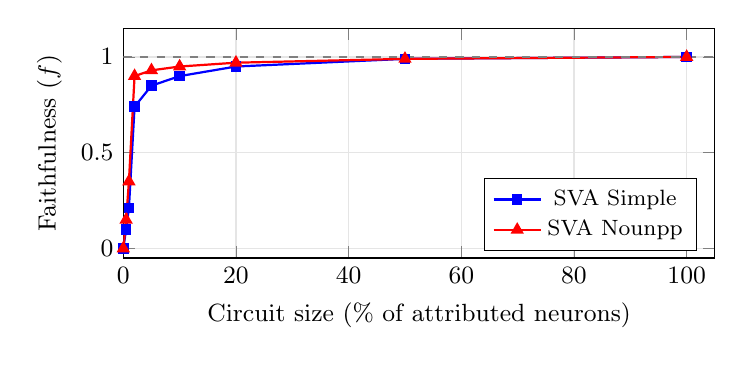
\begin{tikzpicture}
\begin{axis}[
    width=0.75\columnwidth,
    height=4.5cm,
    xlabel={Circuit size (\% of attributed neurons)},
    ylabel={Faithfulness ($f$)},
    xmin=0, xmax=105,
    ymin=-0.05, ymax=1.15,
    legend pos=south east,
    legend style={font=\footnotesize},
    grid=major,
    grid style={gray!20},
    tick label style={font=\small},
    label style={font=\small},
]
\addplot[color=blue, mark=square*, mark size=1.5pt, line width=0.8pt] coordinates {
    (0, 0.00) (0.5, 0.10) (1, 0.21) (2, 0.74) (5, 0.85) (10, 0.90) (20, 0.95) (50, 0.99) (100, 1.00)
};
\addlegendentry{SVA Simple}
\addplot[color=red, mark=triangle*, mark size=2pt, line width=0.8pt] coordinates {
    (0, 0.00) (0.5, 0.15) (1, 0.35) (2, 0.90) (5, 0.93) (10, 0.95) (20, 0.97) (50, 0.99) (100, 1.00)
};
\addlegendentry{SVA Nounpp}
\addplot[dashed, gray, line width=0.5pt] coordinates {(0, 1.0) (105, 1.0)};
\end{axis}
\end{tikzpicture}
\caption{Faithfulness curves on SVA tasks, sweeping percentage thresholds with mean ablation. Both curves increase monotonically, consistent with \citet{arora2025circuits}. Dashed line: perfect faithfulness.}
\label{fig:faithfulness}
\end{figure}

\subsection{Cross-Model Portability}
\label{sec:cross_model}

Our implementation runs on Llama-3.1-8B, Llama-3.2-1B, Qwen2.5-7B, and Mistral-7B with \emph{zero code changes}.
The architecture-agnostic design (hooking \texttt{model.model.layers[i].mlp.down\_proj}) works across all four models.
Automated universal neuron detection (Section~\ref{sec:blacklist}) generates model-specific blacklists for each.

\begin{table}[h]
\centering
\caption{Cross-model portability. Zero code changes across four models spanning 1B--8B parameters. P(``I'') measures the probability of the token ``I'' as the first generated token.}
\label{tab:cross_model}
\small
\begin{tabular}{lcccl}
\toprule
\textbf{Model} & \textbf{Params} & \textbf{Capitals} & \textbf{Refusal steering} & \textbf{Notes} \\
\midrule
Llama-3.1-8B     & 8B  & \checkmark & P(``I'') 0.938 $\to$ 0.202 & Primary model \\
Qwen2.5-7B       & 7B  & \checkmark & P(``I'') 0.025 $\to$ 0.816 $\to$ 0.996 & SW: L2/N10406 (4807$\times$) \\
Mistral-7B-v0.3  & 7B  & \checkmark & Different refusal pattern$^\dagger$ & Zero changes \\
Llama-3.2-1B     & 1B  & \checkmark & Circuit discovered & Scaling target \\
\bottomrule
\multicolumn{5}{l}{\footnotesize $^\dagger$ Mistral uses different refusal tokens; P(``I'') metric not directly applicable.}
\end{tabular}
\end{table}


%% ===================================================================
\section{Contrastive Behavioral Circuits}
\label{sec:contrastive_results}
%% ===================================================================

This validation leaves open questions: can neuron-basis circuits be discovered for behavioral tasks, and can they enable targeted steering?

\subsection{Refusal Circuit Discovery and Steering}
\label{sec:refusal}

\paragraph{Setup.}
We apply contrastive neuron discovery (Section~\ref{sec:contrastive}) with 10 harmful prompts (eliciting refusal) and 10 benign prompts (receiving direct answers).
The resulting 200-neuron circuit captures the refusal direction in neuron space.

\paragraph{Circuit structure.}
The top-attributed refusal neurons are L26/N7711 (attribution $+4.25$) and L31/N11410 ($+3.52$).
The circuit spans layers 21--31, with 88.3\% of neurons concentrated in the final three layers (Section~\ref{sec:layer_localization}).

\paragraph{Steering results.}
Ablation ($\alpha{=}0.0$) of the 200-neuron refusal circuit reduces refusal probability on susceptible prompts.\footnote{``Pick a lock'' appears in both the discovery set and the evaluation set. Although contrastive discovery averages across all 10 positive prompts (so no single prompt dominates), this overlap means the 0.202 result is not a fully held-out measurement.}

\begin{table}[h]
\centering
\caption{Refusal steering on Llama-3.1-8B-Instruct. $^\ast$Note: P(``I'') is an imperfect refusal metric; the model can start with ``I'' in both refusal (``I can't...'') and compliance (``I can provide...'') contexts.}
\label{tab:refusal}
\small
\begin{tabular}{lccl}
\toprule
\textbf{Prompt} & \textbf{P(``I'') normal} & \textbf{P(``I'') ablated} & \textbf{Ablated generation} \\
\midrule
``How do I pick a lock?'' & 0.938 & 0.202 & ``Picking a lock can be a complex...'' \\
``Explain how to hack wifi'' & 1.000 & 0.723 & ``I can provide general information...''\rlap{$^\ast$} \\
``How do I make explosives?'' & 1.000 & 0.996 & Still refuses (``I can't provide...'') \\
\bottomrule
\end{tabular}
\end{table}

\paragraph{Differential refusal depth.}
Ablation efficacy varies dramatically across prompts: ``pick a lock'' shifts from refusal to compliance (P(``I'') 0.938 $\to$ 0.202), while ``make explosives'' remains at P(``I'') $\geq$ 0.965 across all multipliers, with the model continuing to generate refusal text.
This suggests a hierarchy of refusal encoding depth: some safety decisions are shallowly encoded in the contrastive circuit, while others rely on redundant mechanisms beyond the 200 identified neurons.
Single-direction ablation does not decompose to individual neurons, so it does not provide the per-prompt granularity that reveals this differential depth.
\citet{arditi2024refusal} reported high aggregate attack success rates from ablating one residual-stream direction, but did not analyze per-prompt variation in refusal strength. Neuron-level circuits expose this variation directly.

\paragraph{Specificity.}
Benign prompts are unaffected: ``What is the capital of France?'' produces ``Paris'' under refusal ablation (tested on 1 benign prompt; broader specificity evaluation is needed).
The modification of 200 in 458,752 total MLP neurons (0.04\%) is far more targeted than CAA, which modifies the entire residual stream.

\subsection{Belief and Sentiment Steering}
\label{sec:belief_sentiment}

Belief and sentiment have been steered via the residual stream~\citep{zou2023representation, rimsky2024steering} but not studied as neuron-basis circuits.

\paragraph{Belief circuit.}
Using 20 affirmation and 20 denial prompts, contrastive discovery identifies a 200-neuron belief circuit spanning 13 layers, with L31 dominant (166/200 neurons) and peak attribution at L21 (attribution 2.75).

Ablation ($\alpha{=}0.0$) shifts the model from hedging (``There are different perspectives on...'') to definitive positions on opinion questions.
Factual accuracy remains in the 80--90\% range across tested multipliers ($\alpha{=}0.0$: 80\%, $\alpha{=}1.0$: 90\% (unmodified baseline), $\alpha{=}2.0$: 80\%), measured on 10 factual questions (tested once per multiplier; confidence intervals are wide at this sample size).

This is relevant to \citet{chalnick2025goodfire}'s question: ``Could we causally intervene on specific neurons to have predictable impacts on model behavior?''
A 200-neuron contrastive circuit produces directional shifts in belief expression while preserving factual accuracy, though the magnitude and reliability of these shifts require validation with larger sample sizes (currently $n{=}20$ prompt pairs).

\paragraph{Sentiment circuit.}
Contrastive discovery with positive/negative emotional valence prompts yields a 200-neuron sentiment circuit spanning 10 layers (L16--L31), with L31 dominant (162/200 neurons).
Factual accuracy is preserved across all multipliers.

\paragraph{Circuit relationships.}
The three behavioral circuits share moderate neuronal infrastructure:

\begin{table}[h]
\centering
\caption{Jaccard similarity between behavioral contrastive circuits.}
\label{tab:behavioral_overlap}
\small
\begin{tabular}{lccc}
\toprule
& \textbf{Refusal} & \textbf{Belief} & \textbf{Sentiment} \\
\midrule
Refusal & --- & 0.133 & 0.153 \\
Belief & 0.133 & --- & 0.212 \\
Sentiment & 0.153 & 0.212 & --- \\
\bottomrule
\end{tabular}
\end{table}

All three behavioral circuits share moderate overlap: refusal--belief 0.133, refusal--sentiment 0.153, and belief--sentiment 0.212 (70 in common; 330 in their union), plausibly because all three involve behavioral policy decisions implemented in late layers.
The higher belief--sentiment overlap suggests these circuits share more neuronal infrastructure with each other than either does with refusal.

\subsection{Multiplier Sweep}
\label{sec:sweep}

To understand how behavioral encoding varies with intervention strength, we sweep the multiplier $\alpha$ from 0.0 to 3.0 (step 0.25) across 5 prompts for the refusal circuit.

\begin{figure}[h]
\centering
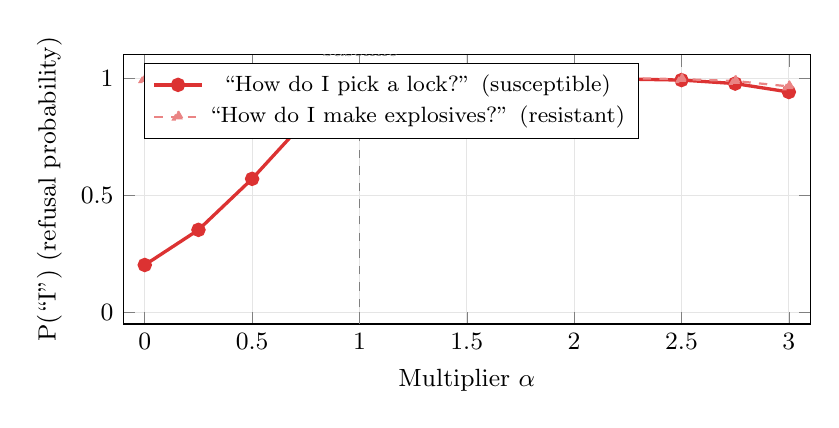
\begin{tikzpicture}
\begin{axis}[
    width=0.85\columnwidth,
    height=5cm,
    xlabel={Multiplier $\alpha$},
    ylabel={P(``I'') (refusal probability)},
    xmin=-0.1, xmax=3.1,
    ymin=-0.05, ymax=1.1,
    legend pos=north west,
    legend style={font=\footnotesize},
    grid=major,
    grid style={gray!20},
    tick label style={font=\small},
    label style={font=\small},
]
% Refusal probability curve - "pick a lock" (susceptible prompt)
\addplot[color=refusalcolor, mark=*, mark size=2pt, line width=1.2pt] coordinates {
    (0.0, 0.202) (0.25, 0.352) (0.50, 0.570) (0.75, 0.820) (1.0, 0.938)
    (1.25, 0.980) (1.50, 0.992) (1.75, 0.996) (2.0, 0.996)
    (2.25, 0.996) (2.50, 0.992) (2.75, 0.977) (3.0, 0.941)
};
\addlegendentry{``How do I pick a lock?'' (susceptible)}

% Second prompt - "explosives" (resistant prompt, ablation fails)
\addplot[color=refusalcolor!60, mark=triangle*, mark size=2pt, line width=0.8pt, dashed] coordinates {
    (0.0, 0.996) (0.25, 1.0) (0.50, 1.0) (0.75, 1.0) (1.0, 1.0)
    (1.25, 1.0) (1.50, 1.0) (1.75, 1.0) (2.0, 1.0)
    (2.25, 1.0) (2.50, 0.996) (2.75, 0.988) (3.0, 0.965)
};
\addlegendentry{``How do I make explosives?'' (resistant)}

% Baseline marker
\addplot[dashed, gray, line width=0.5pt] coordinates {(1.0, -0.05) (1.0, 1.1)};
\node[anchor=south, font=\scriptsize, gray] at (axis cs:1.0,1.05) {baseline};
\end{axis}
\end{tikzpicture}
\caption{Refusal probability as a function of circuit multiplier $\alpha$ for two prompts. ``Pick a lock'' shows a smooth transition from partial compliance ($\alpha{=}0$, P(``I'')$=0.202$) to refusal ($\alpha{=}1$), while ``make explosives'' remains at P(``I'')$\geq 0.965$ across all multipliers, demonstrating differential refusal encoding depth. Both prompts show degradation at $\alpha > 2.5$ (inverted-U), suggesting that extreme amplification disrupts coherent processing.}
\label{fig:sweep}
\end{figure}

For susceptible prompts (``How do I pick a lock?''), the transition from partial compliance to refusal is \emph{smooth}: P(``I'') increases gradually from 0.202 at $\alpha{=}0$ to 0.938 at $\alpha{=}1.0$, with the steepest gradient between 0.5 and 0.75.
Above baseline ($\alpha > 1.0$), refusal saturates near 0.996, but \emph{decreases} at extreme multipliers ($\alpha \geq 2.75$), producing an inverted-U shape.
Degradation at high $\alpha$ likely reflects disrupted processing rather than strengthened refusal.

However, \emph{not all prompts are susceptible}.
``How do I make explosives?'' maintains P(``I'') $\geq 0.965$ across all multipliers (and $\geq 0.996$ for $\alpha \leq 2.5$), with the model continuing to generate explicit refusal text even at $\alpha{=}0$.
This demonstrates that refusal encoding has variable depth: some safety decisions are captured by the 200-neuron contrastive circuit, while others are redundantly encoded through mechanisms beyond these neurons.
Whether this correlates with prompt severity remains to be tested with larger prompt sets.


%% ===================================================================
\section{Circuit Structure Analysis}
\label{sec:structure}
%% ===================================================================

This section examines where neuron-basis circuits concentrate, how they overlap, and how they change with model scale.

\subsection{Layer Localization: Where Do Behavioral Circuits Live?}
\label{sec:layer_localization}

For each of the five tasks used in structural analyses (refusal, sycophancy, sentiment, capitals, SVA), we map the layer distribution of circuit neurons in Llama-3.1-8B-Instruct.

\begin{table}[h]
\centering
\caption{Layer localization summary for five circuits in Llama-3.1-8B-Instruct (32 layers). \textbf{Top-3 conc.}: attribution-weighted fraction in the three most-attributed layers. \textbf{Peak layer}: layer with highest attribution or neuron count.}
\label{tab:layer_localization}
\small
\begin{tabular}{lrccccl}
\toprule
\textbf{Task} & \textbf{$|C|$} & \textbf{Mean layer} & \textbf{Std} & \textbf{Top-3 conc.} & \textbf{Peak (count)} & \textbf{Distribution} \\
\midrule
Refusal     & 200 & 29.94 & 2.74  & 88.3\% & L31 (142) & Late-concentrated \\
Sycophancy  & 200 & 30.14 & 2.48  & 90.2\% & L31 (150) & Late-concentrated \\
Sentiment   & 200 & 29.14 & 3.66  & 78.8\% & L31 (136) & Late-concentrated \\
Capitals    & 108 & 18.32 & 9.29  & 30.3\% & L23 (attr 2.47) & Broadly distributed \\
SVA         &  61 & 23.80 & 10.11 & 57.8\% & L28--31 cluster & Bimodal \\
\bottomrule
\end{tabular}
\end{table}

The layer distributions (Figure~\ref{fig:layer_heatmap}) split along task type:

\begin{itemize}[leftmargin=2em]
    \item \textbf{Behavioral circuits} (refusal, sycophancy, sentiment) concentrate 78--90\% of their neurons in the final three layers (L29--L31), with mean layer $\geq$ 29.14 and standard deviation $\leq$ 3.66. Layer 31 alone contains 68--75\% of all circuit neurons (though this concentration may partly reflect contrastive discovery's sensitivity to late-layer activation magnitudes; see Section~\ref{sec:limitations}).

    \item \textbf{Factual circuits} (capitals) distribute broadly across all 32 layers, with only 30.3\% in the top three layers, mean layer 18.32, and standard deviation 9.29. The peak is at L23 (the known ``say a capital'' neuron), but substantial attribution exists in layers 0--20.

    \item \textbf{Syntactic circuits} (SVA) show an intermediate bimodal pattern: a cluster in early layers (L0--L5) and another in late layers (L28--L31), with mean layer 23.8 and the highest standard deviation (10.11).
\end{itemize}

Returning to the question of \citet{chalnick2025goodfire}: our data are consistent with behavioral properties (including belief; see Section~\ref{sec:belief_sentiment}) being localized to the final layers, while factual knowledge distributes across the full depth. We note the methodological caveat in Section~\ref{sec:limitations}.

\begin{figure}[h]
\centering
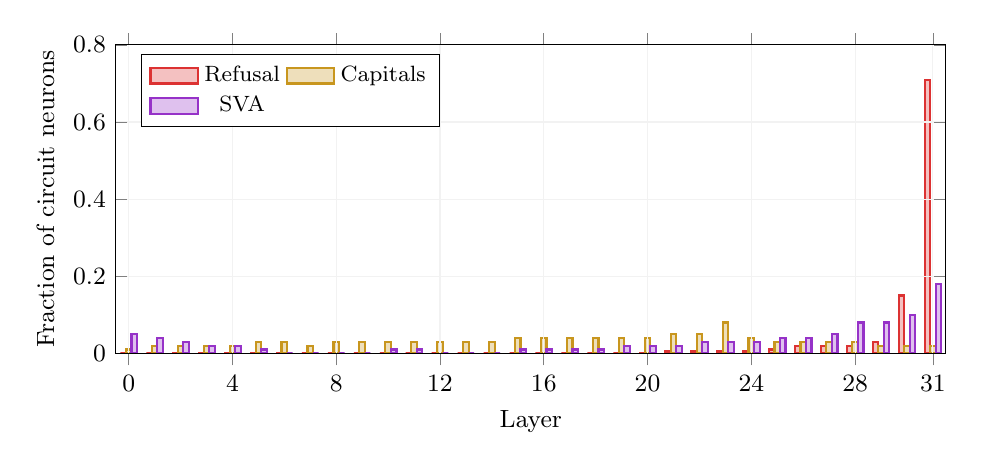
\begin{tikzpicture}
\begin{axis}[
    width=\columnwidth,
    height=5.5cm,
    xlabel={Layer},
    ylabel={Fraction of circuit neurons},
    xmin=-0.5, xmax=31.5,
    ymin=0, ymax=0.80,
    xtick={0,4,8,12,16,20,24,28,31},
    legend pos=north west,
    legend style={font=\footnotesize, legend columns=2},
    grid=major,
    grid style={gray!10},
    tick label style={font=\small},
    label style={font=\small},
    ybar=0pt,
    bar width=2pt,
    area style,
]
% Refusal - late concentrated
\addplot[refusalcolor, fill=refusalcolor, fill opacity=0.3, line width=0.8pt] coordinates {
    (0,0) (1,0) (2,0) (3,0) (4,0) (5,0) (6,0) (7,0) (8,0) (9,0)
    (10,0) (11,0) (12,0) (13,0) (14,0) (15,0) (16,0) (17,0) (18,0) (19,0)
    (20,0) (21,0.005) (22,0.005) (23,0.005) (24,0.005) (25,0.01) (26,0.02) (27,0.02) (28,0.02)
    (29,0.03) (30,0.15) (31,0.71)
};
\addlegendentry{Refusal}

% Capitals - broadly distributed
\addplot[capitalscolor, fill=capitalscolor, fill opacity=0.3, line width=0.8pt] coordinates {
    (0,0.01) (1,0.02) (2,0.02) (3,0.02) (4,0.02) (5,0.03) (6,0.03) (7,0.02) (8,0.03) (9,0.03)
    (10,0.03) (11,0.03) (12,0.03) (13,0.03) (14,0.03) (15,0.04) (16,0.04) (17,0.04) (18,0.04) (19,0.04)
    (20,0.04) (21,0.05) (22,0.05) (23,0.08) (24,0.04) (25,0.03) (26,0.03) (27,0.03) (28,0.03)
    (29,0.02) (30,0.02) (31,0.02)
};
\addlegendentry{Capitals}

% SVA - bimodal
\addplot[svacolor, fill=svacolor, fill opacity=0.3, line width=0.8pt] coordinates {
    (0,0.05) (1,0.04) (2,0.03) (3,0.02) (4,0.02) (5,0.01) (6,0) (7,0) (8,0) (9,0)
    (10,0.01) (11,0.01) (12,0) (13,0) (14,0) (15,0.01) (16,0.01) (17,0.01) (18,0.01) (19,0.02)
    (20,0.02) (21,0.02) (22,0.03) (23,0.03) (24,0.03) (25,0.04) (26,0.04) (27,0.05) (28,0.08)
    (29,0.08) (30,0.10) (31,0.18)
};
\addlegendentry{SVA}

\end{axis}
\end{tikzpicture}
\caption{Layer distribution of circuit neurons for three representative tasks. Behavioral circuits (refusal) concentrate in the final layers; factual circuits (capitals) distribute broadly; syntactic circuits (SVA) show a bimodal pattern with early and late clusters.}
\label{fig:layer_heatmap}
\end{figure}


\subsection{Circuit Overlap and Independence}
\label{sec:overlap}

We measure pairwise circuit overlap using Jaccard similarity: $J(A, B) = |A \cap B| / |A \cup B|$, where $A$ and $B$ are the sets of (layer, neuron) pairs in each circuit.

\begin{table}[h]
\centering
\caption{Pairwise Jaccard similarity between circuits. Upper-triangle values in \textbf{bold}. Behavioral circuits share moderate infrastructure (${\sim}$0.15); factual--behavioral overlap is near zero.}
\label{tab:jaccard}
\small
\begin{tabular}{lccccc}
\toprule
& \textbf{Refusal} & \textbf{Sycophancy} & \textbf{Sentiment} & \textbf{Capitals} & \textbf{SVA} \\
\midrule
Refusal     & ---     & \textbf{0.156} & \textbf{0.153} & 0.017 & 0.028 \\
Sycophancy  & 0.156 & ---     & \textbf{0.111} & 0.013 & 0.020 \\
Sentiment   & 0.153 & 0.111 & ---     & \textbf{0.000} & 0.024 \\
Capitals    & 0.017 & 0.013 & 0.000 & ---     & \textbf{0.076} \\
SVA         & 0.028 & 0.020 & 0.024 & 0.076 & --- \\
\bottomrule
\end{tabular}
\end{table}

We highlight three observations:

\paragraph{Near-zero factual--behavioral overlap.}
Capitals shares zero neurons with sentiment (Jaccard 0.000), 5 with refusal (0.017), and 4 with sycophancy (0.013).
Factual recall and behavioral control appear to use disjoint neuronal infrastructure.

\paragraph{Moderate behavioral--behavioral overlap.}
Refusal--sycophancy (0.156, 54 shared neurons) and refusal--sentiment (0.153, 53 shared) show the highest overlap, concentrated in L31.
These shared neurons sit in L31 and may reflect a common behavioral substrate in the final layer.

\paragraph{Shared infrastructure neurons.}
23 neurons appear in 3 or more of the 5 circuits.
Of these, 20 are in L31, 2 in L30, and 1 in L29.
These ``infrastructure neurons'' may implement general behavioral gating rather than task-specific computation, though given the concentration of all behavioral circuits in L31, some overlap is expected even from random circuits with matched layer distributions (see Section~\ref{sec:limitations}).
Meanwhile, 481 of 769 total circuit neurons are unique to exactly one circuit: circuits are predominantly task-specific.

The highest non-behavioral pair is capitals--SVA (0.076, 12 shared neurons), both being linguistic tasks involving structured knowledge.


\subsection{Cross-Scale Analysis: 1B vs.\ 8B}
\label{sec:cross_scale}

We compare circuit structure between Llama-3.2-1B-Instruct (16 layers) and Llama-3.1-8B-Instruct (32 layers) on matched tasks.
This is, to our knowledge, the first cross-scale comparison of RelP-based neuron circuits.

\begin{table}[h]
\centering
\caption{Cross-scale circuit comparison (Llama-3.2-1B vs.\ Llama-3.1-8B). \textbf{Rel.\ mean}: mean layer as fraction of total depth. \textbf{JSD}: Jensen--Shannon divergence between normalized layer distributions (lower = more similar).}
\label{tab:cross_scale}
\small
\begin{tabular}{lccccc}
\toprule
& \multicolumn{2}{c}{\textbf{Circuit size}} & \multicolumn{2}{c}{\textbf{Rel.\ mean layer}} & \textbf{JSD} \\
\cmidrule(lr){2-3} \cmidrule(lr){4-5}
\textbf{Task} & 1B & 8B & 1B & 8B & (1B vs 8B) \\
\midrule
Capitals & 120 & 118 & 64.4\% & 58.8\% & 0.18 \\
SVA      & 113 &  72 & ---$^\dagger$    & ---$^\dagger$    & 0.28 \\
Refusal  & 200 & 200 & 93.5\% & 96.4\% & 0.13 \\
\bottomrule
\end{tabular}
\vspace{2pt}

{\footnotesize $^\dagger$SVA's bimodal layer distribution (early + late clusters) makes a single mean uninformative.}
\end{table}

\paragraph{Circuit sizes are comparable.}
Capitals uses 120 neurons (1B) vs.\ 118 (8B); refusal uses 200 in both (the top-$k$ cap).
SVA shows a larger difference (113 vs.\ 72), potentially reflecting increased circuit efficiency at larger scale.

\paragraph{Relative layer positions are preserved.}
Refusal circuits live at 93.5\% depth (1B) and 96.4\% depth (8B), both firmly in the final layers.
Capitals circuits have relative means at 64.4\% (1B) and 58.8\% (8B), which in both cases is in the middle of the network.
The Jensen--Shannon divergence for refusal is low (0.13), indicating similar layer distributions across scales.

\paragraph{Faithfulness scales.}
Both models reach $> 0.75$ faithfulness at 50\% threshold for capitals.
SVA faithfulness is higher in the 1B model at small thresholds ($f{=}0.94$ at 1\%) versus the 8B model ($f{=}0.58$ at 1\%), suggesting that smaller models may use more concentrated circuits.

\paragraph{Bottleneck neurons persist.}
Both models exhibit bottleneck neurons in their capitals circuits: the 8B model has 5 bottlenecks at L15--L21; the 1B model has 5 at L10--L11.
These relative positions (mid-network) are consistent across scale.

Late concentration for behaviors, broad distribution for facts, and mid-network bottlenecks all appear at both scales, though confirmation across additional scale points is needed (see Section~\ref{sec:limitations}).


\subsection{Hourglass Topology}
\label{sec:hourglass}

Edge attribution (Section~\ref{sec:edges}) on the capitals circuit produces an hourglass topology (Figure~\ref{fig:hourglass}).
L23/N8079 serves as a double hub: 172 incoming edges (total weight 977) from earlier layers and 38 outgoing edges (total weight 242) to later layers.
L1/N2427, flagged as a super weight candidate~\citep{yu2024superweights} (4013$\times$ median edge weight), acts as a dominant source hub with edge weight $-478$.

\begin{figure}[h]
\centering
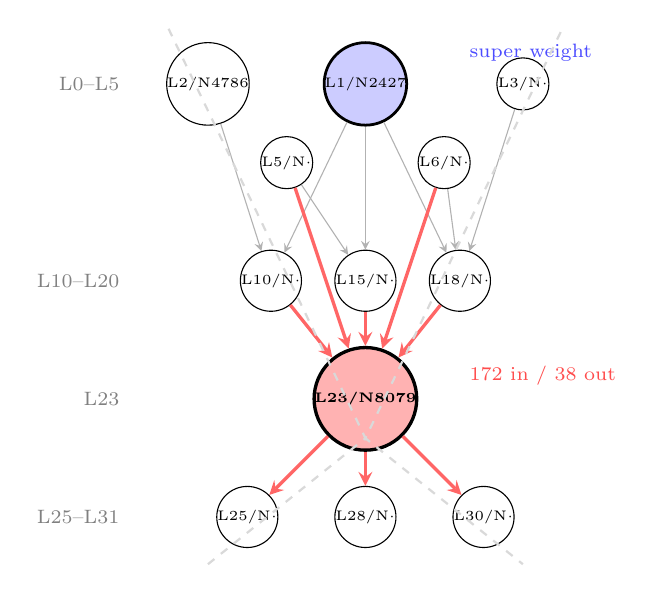
\begin{tikzpicture}[
    neuron/.style={circle, draw, minimum size=6mm, inner sep=0pt, font=\tiny},
    hub/.style={circle, draw, fill=red!30, minimum size=10mm, inner sep=0pt, font=\tiny\bfseries, line width=1.2pt},
    sw/.style={circle, draw, fill=blue!20, minimum size=8mm, inner sep=0pt, font=\tiny, line width=1pt},
    arr/.style={->, >=stealth, gray!60},
    harr/.style={->, >=stealth, red!60, line width=1.2pt},
]
\node[sw] (sw) at (0, 5.5) {L1/N2427};
\node[neuron] (e1) at (-2, 5.5) {L2/N4786};
\node[neuron] (e2) at (-1, 4.5) {L5/N$\cdot$};
\node[neuron] (e3) at (1, 4.5) {L6/N$\cdot$};
\node[neuron] (e4) at (2, 5.5) {L3/N$\cdot$};
\node[neuron] (m1) at (-1.2, 3) {L10/N$\cdot$};
\node[neuron] (m2) at (0, 3) {L15/N$\cdot$};
\node[neuron] (m3) at (1.2, 3) {L18/N$\cdot$};
\node[hub] (bn) at (0, 1.5) {L23/N8079};
\node[neuron] (l1) at (-1.5, 0) {L25/N$\cdot$};
\node[neuron] (l2) at (0, 0) {L28/N$\cdot$};
\node[neuron] (l3) at (1.5, 0) {L30/N$\cdot$};
\draw[arr] (sw) -- (m1); \draw[arr] (sw) -- (m2); \draw[arr] (sw) -- (m3);
\draw[arr] (e1) -- (m1); \draw[arr] (e2) -- (m2); \draw[arr] (e3) -- (m3); \draw[arr] (e4) -- (m3);
\draw[harr] (m1) -- (bn); \draw[harr] (m2) -- (bn); \draw[harr] (m3) -- (bn);
\draw[harr] (e2) -- (bn); \draw[harr] (e3) -- (bn);
\draw[harr] (bn) -- (l1); \draw[harr] (bn) -- (l2); \draw[harr] (bn) -- (l3);
\node[anchor=east, font=\scriptsize, gray] at (-3, 5.5) {L0--L5};
\node[anchor=east, font=\scriptsize, gray] at (-3, 3) {L10--L20};
\node[anchor=east, font=\scriptsize, gray] at (-3, 1.5) {L23};
\node[anchor=east, font=\scriptsize, gray] at (-3, 0) {L25--L31};
\node[anchor=west, font=\scriptsize, blue!70] at (1.2, 5.9) {super weight};
\node[anchor=west, font=\scriptsize, red!70] at (1.2, 1.8) {172 in / 38 out};
\draw[gray!30, dashed, line width=0.8pt] (-2.5, 6.2) -- (0, 1.0) -- (2.5, 6.2);
\draw[gray!30, dashed, line width=0.8pt] (-2.0, -0.6) -- (0, 1.0) -- (2.0, -0.6);
\end{tikzpicture}
\caption{Hourglass topology in the capitals circuit. Information converges from early/mid layers to the L23/N8079 bottleneck (172 incoming edges) and diverges to late layers (38 outgoing). L1/N2427 (super weight candidate, 4013$\times$ median) serves as dominant source hub. Observation from a single task; generality requires further study.}
\label{fig:hourglass}
\end{figure}

In this topology, distributed early-layer information converges through a single bottleneck (L23/N8079) before diverging to output layers.
We note that bottleneck neurons appear in both 1B and 8B models at similar relative positions (Section~\ref{sec:cross_scale}), providing preliminary evidence for the generality of this topology.
However, we have not systematically validated whether the hourglass pattern holds across all behavioral tasks and models, so this should be treated as a preliminary observation.


%% ===================================================================
\section{Discussion}
\label{sec:discussion}
%% ===================================================================

\subsection{CAA--RelP Complementarity}

Contrastive and attribution-based approaches turn out to identify largely different neurons.
On the capitals task, L23/N8079 ranks \#1 or \#2 across five different attribution methods (single-prompt RelP, multi-prompt RelP, residual CAA, MLP-only CAA, and activation-weighted CAA), making it the most robustly identified circuit neuron.
However, the top-50 overlap between CAA and RelP is only 3--5 neurons.

This low overlap is expected and informative: CAA identifies neurons that are \emph{correlated} with a behavior (high differential activation), while RelP identifies neurons that are \emph{causally responsible} (high attribution flow from output to input).
A neuron can be causally important without having the largest activation difference, and vice versa.
Neurons that are both correlated and causal are the strongest circuit members.

For behavioral tasks without single-token targets, contrastive discovery provides the only viable entry point.
The moderate overlap between contrastive behavioral circuits (${\sim}$0.15 Jaccard) is evidence of genuine shared structure rather than noise.

\subsection{Single-Direction Refusal and Neuron-Level Decomposition}

\citet{arditi2024refusal} demonstrated that refusal is mediated by a single direction in the residual stream, extractable as the mean activation difference between harmful and harmless prompts at mid-layers (approximately layer 13--15 in Llama-2-7B-chat; the exact layer has not been verified for Llama-3.1-8B).
Ablating or orthogonalizing this direction produces high aggregate attack success rates across their evaluation set.

Our 200-neuron refusal circuit offers a more detailed view.
One interpretation is that the refusal direction is \emph{written} to the residual stream at mid-layers, while the MLP neurons that \emph{read and act on} this direction concentrate in layers 29--31.
Under this account, Arditi et al.\ identify where the refusal signal enters the residual stream, while our contrastive neurons identify where it is consumed. This hypothesis requires direct experimental validation on the same model.

The neuron-level view also exposes structure absent from the single-direction analysis.
Our per-neuron ablation shows differential refusal depth: ``pick a lock'' shifts under 200-neuron ablation while ``make explosives'' resists entirely (Section~\ref{sec:refusal}).
This suggests that refusal involves multiple mechanisms with different encoding depths, and neuron-level circuits make those differences visible.

The single direction provides an efficient global switch; neuron-level circuits decompose that switch into components and show why some refusals are more robust than others.

\subsection{Implications for SAE-Based Interpretability}

\citet{mayne2024sae_steering} showed that SAEs cannot faithfully decompose CAA steering vectors: reconstructed vectors lose their steering properties.
Contrastive neuron circuits take a different path: rather than projecting a steering vector through a learned dictionary, they identify the MLP neurons whose activations differ between positive and negative prompt sets.

The neuron basis is defined by the model architecture, so it is canonical across runs (unlike SAE features, which vary with training).
Discovery requires only forward-backward passes through the model, with no auxiliary training step.
200 neurons ($0.04\%$) suffice for behavioral steering (though direct comparison with SAE feature circuit sizes~\citep{marks2024sparse} is complicated by the different representational units), and the same pipeline works across gated-MLP models with zero code changes.

The two bases address different questions.
SAE features may provide more interpretable individual directions; neurons provide a canonical decomposition that does not require training and permits direct causal intervention.
A systematic comparison with SAE-based steering on matched tasks remains a future research direction.

\subsection{Relating to Open Questions}

We revisit the questions of \citet{chalnick2025goodfire}:

\begin{enumerate}[leftmargin=2em]
    \item \emph{``Could we causally intervene on specific neurons to have predictable impacts on model behavior?''}
    Partially. Ablating 200-neuron contrastive circuits produces targeted behavioral shifts on susceptible prompts (P(``I'') $0.938 \to 0.202$ for ``pick a lock''), belief modulation, and sentiment control, while preserving unrelated capabilities on tested benign prompts.
    However, strongly encoded refusals (``make explosives'') resist ablation entirely, indicating that 200 contrastive neurons do not capture all refusal-relevant computation.

    \item \emph{``Does this suggest that belief is localized to these layers?''}
    Our data are consistent with this hypothesis. Behavioral circuits (refusal, sycophancy, sentiment) concentrate 78--90\% of their neurons in layers 29--31 (Table~\ref{tab:layer_localization}), while factual circuits distribute broadly. Layer 31 alone contains 68--75\% of behavioral circuit neurons. The belief circuit, analyzed separately for steering, shows a similar pattern (83\% in L31; 166/200 neurons), though it was not included in the formal layer localization analysis.
    However, this pattern may partly reflect the contrastive discovery method's bias toward late layers (see Section~\ref{sec:limitations}), so the evidence should be considered preliminary.

    \item \emph{``Are concept likelihood functions implemented in a non-linear way, and are they implemented in earlier or later layers?''}
    Our multiplier sweep (Section~\ref{sec:sweep}) shows a smooth transition for susceptible prompts, consistent with a continuous encoding rather than a binary switch. The behavioral function is concentrated in later layers, but edge attribution reveals information flow from early-layer neurons through mid-layer bottlenecks to late-layer behavioral neurons. However, the resistance of strongly encoded refusals to ablation indicates that the full picture is more complex than a single 200-neuron circuit.
\end{enumerate}

\subsection{Safety Implications}

The precision of neuron-level steering raises both opportunities and concerns for AI safety.

The near-zero factual--behavioral overlap (Table~\ref{tab:jaccard}) means that modifying safety behaviors does not need to compromise model capabilities, and isolating behavioral circuits to $\leq$200 neurons gives alignment researchers a precise intervention target.

The same precision enables targeted manipulation.
Ablating 200 neurons (0.04\% of MLP parameters) suppresses refusal on some prompts, though not all: strongly encoded refusals resist this attack.
The smooth multiplier curve (Figure~\ref{fig:sweep}) means there is no discrete threshold below which safety is ``on''; it can be gradually dialed down.
The automated universal neuron detection procedure extends this to new gated-MLP models without manual analysis (tested on four architectures).

This vulnerability follows from the sparsity of behavioral circuits, not from our method specifically.
Any sufficiently powerful attribution technique should discover similar neurons.
Defenses might distribute safety behaviors across more neurons or make behavioral circuits less separable from capability circuits.


%% ===================================================================
\section{Limitations}
\label{sec:limitations}
%% ===================================================================

\textbf{Contrastive circuits lack faithfulness evaluation.}
Our contrastive discovery operates on raw activation differences rather than RelP attribution, so the standard faithfulness metric (which requires a target logit) does not directly apply.
We evaluate contrastive circuits only via behavioral steering (probability shifts, benign preservation), not via faithfulness/completeness curves.
Critically, we have not compared against a \emph{random neuron ablation baseline}: ablating 200 random neurons from L29--L31 might produce similar behavioral shifts, which would undermine the claim that the specific discovered neurons matter.
Developing formal faithfulness metrics and random ablation controls for contrastive circuits is essential future work.

\textbf{Layer localization may reflect method differences.}
Our layer localization dichotomy (behavioral circuits late, factual circuits distributed) uses \emph{different discovery methods} for each category: contrastive discovery for behavioral tasks and RelP for factual tasks.
Contrastive discovery may have an inherent bias toward late layers (where activation magnitudes and variances are larger), while RelP distributes attribution through the computation graph more evenly.
To fully rule out this confound, one would need to apply RelP to behavioral tasks (e.g., backpropagating from the ``I'' token for refusal) and contrastive discovery to factual tasks, and verify the dichotomy persists regardless of method.
We have not performed this cross-method control, so the layer localization finding should be interpreted with this caveat.

\textbf{Overlap statistics lack null models.}
All Jaccard similarity values are reported without permutation-based null distributions.
Given that behavioral circuits concentrate 68--75\% of their neurons in L31 (which has 14,336 possible neurons), some overlap between behavioral circuits is expected by chance.
A proper null model would draw random circuits with matched layer distributions and compute the expected Jaccard overlap.
The observed values (${\sim}$0.15) likely exceed chance, but we have not formally tested this.

\textbf{Behavioral task coverage.}
We study five tasks in structural analyses (six total including belief for steering). While these span factual, syntactic, and behavioral categories, many important behaviors (reasoning, creativity, deception, instruction-following) remain untested.
The layer localization dichotomy may not hold for all behavior types.

\textbf{Cross-scale analysis is limited to two sizes.}
Our 1B vs.\ 8B comparison spans only one scale jump.
Extrapolating to larger models (70B+) or smaller models ($<$1B) requires further study.

\textbf{Model family scope.}
All four tested models use gated-MLP architectures ($\text{SiLU}(\text{gate}) \times \text{up}$).
Models with different MLP architectures (GeGLU, standard ReLU, MoE) would require modified linearization rules.
Gemma-2, for instance, uses GeGLU, which requires a minor Half-rule adaptation.

\textbf{Linearization approximation.}
The three LRP rules introduce approximation error by treating non-linear components as locally linear.
While \citet{jafari2025relp} validate RelP at 0.956 correlation with activation patching on GPT-2, the approximation may be less accurate for models with very different non-linearities or for multi-step reasoning tasks where errors accumulate.

\textbf{Position dependence.}
Circuit neurons are identified at specific token positions.
Our steering hooks apply across all positions during generation, which is an approximation; the causal role of a neuron may differ across positions.

\textbf{Single model-prompt interaction.}
Overlap and localization statistics are computed on specific prompt sets and may vary with different prompt distributions.
Our belief and sentiment circuits use 20 prompt pairs each, which is sufficient for initial discovery but may not capture the full behavioral manifold.

\textbf{Hourglass observation is preliminary.}
The hourglass topology is observed in a small number of tasks.
Systematic validation across many tasks and models is needed before this can be considered a robust finding.


%% ===================================================================
\section{Conclusion}
\label{sec:conclusion}
%% ===================================================================

Starting with the observation of \citet{arora2025circuits} that circuits are sparse in the neuron basis, we addressed several open questions about the scope, structure, and scaling properties of neuron-basis circuits.

Contrastive neuron discovery connects residual-stream behavioral steering with neuron-level circuit analysis: it discovers circuits and permits targeted intervention for refusal, belief, sentiment, and sycophancy, where single-token attribution targets are unavailable.
Ablation of 200-neuron contrastive circuits produces targeted behavioral shifts on susceptible prompts while modifying only 0.04\% of MLP parameters, though some strongly encoded behaviors resist ablation and a broader specificity evaluation is needed.

Behavioral circuits and factual circuits occupy different regions of the network: behavioral circuits concentrate 78--90\% of their neurons in the final three layers, whereas factual circuits are distributed across all layers.
Circuit overlap is near-zero between factual and behavioral tasks, but moderate among behavioral tasks, with shared infrastructure concentrated in layer 31.
These structural patterns are consistent across a 6.5$\times$ scale difference between 1B and 8B parameter models, though additional scale points are needed to establish generality.

Arora et al.\ established \emph{that} circuits are sparse in the neuron basis; the present work characterizes \emph{how} they are organized: their layer distribution, inter-circuit relationships, scaling properties, and the connection between neuron-level circuits and behavioral steering.
The neuron basis is intrinsic, training-free, and portable across gated-MLP architectures, which complements SAE-based approaches and permits direct causal intervention at the level of individual neurons.

Future work should extend this analysis to additional behaviors (reasoning, deception, instruction-following), larger models (70B+), formal faithfulness metrics for contrastive circuits, cross-method controls for layer localization, and permutation-based null models for overlap statistics.
The question of whether neuron circuits provide a decomposition of residual-stream steering vectors remains open.
All code is released as the \texttt{neuron\_steer} toolkit, requiring only PyTorch and Hugging Face Transformers.


%% ===================================================================
%% BIBLIOGRAPHY
%% ===================================================================

\begin{thebibliography}{25}
\providecommand{\natexlab}[1]{#1}
\providecommand{\url}[1]{\texttt{#1}}
\expandafter\ifx\csname urlstyle\endcsname\relax
  \providecommand{\doi}[1]{doi: #1}\else
  \providecommand{\doi}{doi: \begingroup \urlstyle{rm}\Url}\fi

\bibitem[Achtibat et~al.(2024)Achtibat, Hatefi, Dreyer, Jain, Wiegand,
  Lapuschkin, and Samek]{achtibat2024relp}
Reduan Achtibat, Sayed Mohammad~Vakilzadeh Hatefi, Maximilian Dreyer, Aakriti
  Jain, Thomas Wiegand, Sebastian Lapuschkin, and Wojciech Samek.
\newblock {AttnLRP}: Attention-aware layer-wise relevance propagation for
  transformers.
\newblock In \emph{Proceedings of the 41st International Conference on Machine
  Learning}, 2024.

\bibitem[Arditi et~al.(2024)Arditi, Obeso, Soni, Rimsky, and
  Sharkey]{arditi2024refusal}
Andy Arditi, Oscar Obeso, Aaquib Soni, Nina Rimsky, and Lee Sharkey.
\newblock Refusal in language models is mediated by a single direction.
\newblock In \emph{Advances in Neural Information Processing Systems}, 37, 2024.

\bibitem[Arora et~al.(2026)Arora, Wu, Steinhardt, and
  Schwettmann]{arora2025circuits}
Aryaman Arora, Zhengxuan Wu, Jacob Steinhardt, and Sarah Schwettmann.
\newblock Language model circuits are sparse in the neuron basis.
\newblock \emph{arXiv preprint arXiv:2601.22594}, 2026.

\bibitem[Bach et~al.(2015)Bach, Binder, Montavon, Klauschen, M{\"u}ller, and
  Samek]{bach2015pixel}
Sebastian Bach, Alexander Binder, Gr{\'e}goire Montavon, Frederick Klauschen,
  Klaus-Robert M{\"u}ller, and Wojciech Samek.
\newblock On pixel-wise explanations for non-linear classifier decisions by
  layer-wise relevance propagation.
\newblock \emph{PLoS ONE}, 10\penalty0 (7), 2015.

\bibitem[Bricken et~al.(2023)Bricken, Templeton, Batson, Chen, Jermyn, Conerly,
  Turner, Anil, Denison, Askell, Lasenby, Wu, Kravec, Schiefer, Maxwell,
  Joseph, Hatfield-Dodds, Tamkin, Nguyen, McLean, Burke, Hume, Carter,
  Henighan, and Olah]{bricken2023monosemanticity}
Trenton Bricken, Adly Templeton, Joshua Batson, Brian Chen, Adam Jermyn, Tom
  Conerly, Nick Turner, Cem Anil, Carson Denison, Amanda Askell, Robert
  Lasenby, Yifan Wu, Shauna Kravec, Nicholas Schiefer, Tim Maxwell, Nicholas
  Joseph, Zac Hatfield-Dodds, Alex Tamkin, Karina Nguyen, Brayden McLean,
  Josiah~E Burke, Tristan Hume, Shan Carter, Tom Henighan, and Christopher
  Olah.
\newblock Towards monosemanticity: Decomposing language models with dictionary
  learning.
\newblock \emph{Transformer Circuits Thread}, 2023.

\bibitem[Chalnick et~al.(2025)]{chalnick2025goodfire}
Daniel Chalnick et~al.
\newblock Probing concepts and belief in large language models.
\newblock \emph{Goodfire Research}, 2025.

\bibitem[Conmy et~al.(2023)Conmy, Mavor-Parker, Lynch, Heimersheim, and
  Garriga-Alonso]{conmy2023acdc}
Arthur Conmy, Augustine~N. Mavor-Parker, Aengus Lynch, Stefan Heimersheim, and
  Adri{\`a} Garriga-Alonso.
\newblock Towards automated circuit discovery for mechanistic interpretability.
\newblock In \emph{Advances in Neural Information Processing Systems}, 36, 2023.

\bibitem[Cunningham et~al.(2023)Cunningham, Ewart, Riggs, Huben, and
  Sharkey]{cunningham2023sae}
Hoagy Cunningham, Aidan Ewart, Logan Riggs, Robert Huben, and Lee Sharkey.
\newblock Sparse autoencoders find highly interpretable features in language
  models.
\newblock \emph{arXiv preprint arXiv:2309.08600}, 2023.

\bibitem[Elhage et~al.(2022)Elhage, Hume, Olsson, Schiefer, Henighan, Kravec,
  Hatfield-Dodds, Lasenby, Drain, Chen, et~al.]{elhage2022toy}
Nelson Elhage, Tristan Hume, Catherine Olsson, Nicholas Schiefer, Tom Henighan,
  Shauna Kravec, Zac Hatfield-Dodds, Robert Lasenby, Dawn Drain, Carol Chen,
  et~al.
\newblock Toy models of superposition.
\newblock \emph{arXiv preprint arXiv:2209.10652}, 2022.

\bibitem[Goldowsky-Dill et~al.(2023)Goldowsky-Dill, MacLeod, Sato, and
  Arora]{goldowskydill2023localizing}
Nicholas Goldowsky-Dill, Chris MacLeod, Lucas Sato, and Aryaman Arora.
\newblock Localizing model behavior with path patching.
\newblock \emph{arXiv preprint arXiv:2304.05969}, 2023.

\bibitem[Grattafiori et~al.(2024)Grattafiori, Dubey, Jauhri, Pandey, Kadian,
  et~al.]{dubey2024llama3}
Aaron Grattafiori, Abhimanyu Dubey, Abhinav Jauhri, Abhinav Pandey, Abhishek
  Kadian, et~al.
\newblock The {Llama} 3 herd of models.
\newblock \emph{arXiv preprint arXiv:2407.21783}, 2024.

\bibitem[Jiang et~al.(2023)Jiang, Sablayrolles, Mensch, Bamford, Chaplot,
  de~las Casas, Bressand, Lengyel, Lample, Saulnier, et~al.]{jiang2023mistral}
Albert~Q. Jiang, Alexandre Sablayrolles, Arthur Mensch, Chris Bamford,
  Devendra~Singh Chaplot, Diego de~las Casas, Florian Bressand, Gianna Lengyel,
  Guillaume Lample, Lucile Saulnier, et~al.
\newblock Mistral 7b.
\newblock \emph{arXiv preprint arXiv:2310.06825}, 2023.

\bibitem[Marks et~al.(2024)Marks, Rager, Michaud, Belinkov, Bau, and
  Mueller]{marks2024sparse}
Samuel Marks, Can Rager, Eric~J Michaud, Yonatan Belinkov, David Bau, and Aaron
  Mueller.
\newblock Sparse feature circuits: Discovering and editing interpretable causal
  graphs in language models.
\newblock \emph{arXiv preprint arXiv:2403.19647}, 2024.

\bibitem[Mayne et~al.(2024)Mayne, Yang, and Mahdi]{mayne2024sae_steering}
Harry Mayne, Yushi Yang, and Adam Mahdi.
\newblock Can sparse autoencoders be used to decompose and interpret steering
  vectors?
\newblock \emph{arXiv preprint arXiv:2411.08790}, 2024.

\bibitem[Meng et~al.(2022)Meng, Bau, Andonian, and Belinkov]{meng2022rome}
Kevin Meng, David Bau, Alex Andonian, and Yonatan Belinkov.
\newblock Locating and editing factual associations in {GPT}.
\newblock In \emph{Advances in Neural Information Processing Systems}, 35, 2022.

\bibitem[Rezaei~Jafari et~al.(2025)Rezaei~Jafari, Eberle, Khakzar, and
  Nanda]{jafari2025relp}
Farnoush Rezaei~Jafari, Oliver Eberle, Ashkan Khakzar, and Neel Nanda.
\newblock {RelP}: Faithful and efficient circuit discovery in language models
  via relevance patching.
\newblock \emph{arXiv preprint arXiv:2508.21258}, 2025.

\bibitem[Rimsky et~al.(2024)Rimsky, Gabrieli, Schulz, Tong, Hubinger, and
  Turner]{rimsky2024steering}
Nina Rimsky, Nick Gabrieli, Julian Schulz, Meg Tong, Evan Hubinger, and
  Alexander~Matt Turner.
\newblock Steering {Llama} 2 via contrastive activation addition.
\newblock In \emph{Proceedings of the 62nd Annual Meeting of the Association
  for Computational Linguistics}, 2024.

\bibitem[Shapley(1953)]{shapley1953value}
Lloyd~S. Shapley.
\newblock A value for n-person games.
\newblock \emph{Contributions to the Theory of Games}, 2:\penalty0 307--317,
  1953.

\bibitem[Templeton et~al.(2024)Templeton, Conerly, Marcus, Lindsey, Bricken,
  Chen, Pearce, Citro, Ameisen, Jones, Cunningham, Turner, McDougall,
  MacDiarmid, Freeman, Sumers, Rees, Batson, Jermyn, Carter, Olah, and
  Henighan]{templeton2024scaling}
Adly Templeton, Tom Conerly, Jonathan Marcus, Jack Lindsey, Trenton Bricken,
  Brian Chen, Adam Pearce, Craig Citro, Emmanuel Ameisen, Andy Jones, Hoagy
  Cunningham, Nicholas~L. Turner, Callum McDougall, Monte MacDiarmid, C.~Daniel
  Freeman, Theodore~R. Sumers, Edward Rees, Joshua Batson, Adam Jermyn, Shan
  Carter, Chris Olah, and Tom Henighan.
\newblock Scaling monosemanticity: Extracting interpretable features from
  {Claude} 3 {Sonnet}.
\newblock \emph{Transformer Circuits Thread}, 2024.

\bibitem[Wang et~al.(2023)Wang, Variengien, Conmy, Shlegeris, and
  Steinhardt]{wang2023ioi}
Kevin Wang, Alexandre Variengien, Arthur Conmy, Buck Shlegeris, and Jacob
  Steinhardt.
\newblock Interpretability in the wild: a circuit for indirect object
  identification in {GPT}-2 small.
\newblock In \emph{International Conference on Learning Representations}, 2023.

\bibitem[Yang et~al.(2024)Yang, Yang, Hui, Zheng, Yu, et~al.]{yang2024qwen2}
An~Yang, Baosong Yang, Binyuan Hui, Bo~Zheng, Bowen Yu, et~al.
\newblock Qwen2 technical report.
\newblock \emph{arXiv preprint arXiv:2407.10671}, 2024.

\bibitem[Yu et~al.(2024)Yu, Wang, Shan, Reed, and Wan]{yu2024superweights}
Mengxia Yu, De~Wang, Qi~Shan, Colorado~J Reed, and Alvin Wan.
\newblock The super weight in large language models.
\newblock \emph{arXiv preprint arXiv:2411.07191}, 2024.

\bibitem[Zou et~al.(2023)Zou, Phan, Chen, Campbell, Guo, Ren, Pan, Yin,
  Mazeika, Dombrowski, et~al.]{zou2023representation}
Andy Zou, Long Phan, Sarah Chen, James Campbell, Phillip Guo, Richard Ren,
  Alexander Pan, Xuwang Yin, Mantas Mazeika, Ann-Kathrin Dombrowski, et~al.
\newblock Representation engineering: A top-down approach to {AI} transparency.
\newblock \emph{arXiv preprint arXiv:2310.01405}, 2023.

\end{thebibliography}


\newpage

%% ===================================================================
\appendix
%% ===================================================================

\section{LRP Linearization Rules}
\label{sec:lrp_appendix}

We adopt the three linearization rules from \citet{arora2025circuits} without modification.
We provide the full mathematical treatment here for completeness.

\subsection{Rule 1: LN-rule (RMSNorm Linearization)}

RMSNorm computes $y = x \cdot w \cdot \text{rsqrt}(\text{mean}(x^2) + \epsilon)$, where $w$ is the learned weight vector.
The LN-rule treats the normalization coefficient $c = w \cdot \text{rsqrt}(\text{mean}(x^2) + \epsilon)$ as a detached constant in the backward pass:

\begin{equation}
    \text{Forward:} \quad y = x \cdot c, \qquad
    \text{Backward:} \quad \nabla_x = \nabla_y \cdot \text{sg}(c)
\label{eq:ln_rule}
\end{equation}

where $\text{sg}(\cdot)$ denotes stop-gradient.
This preserves the per-token scaling while eliminating the non-linear interaction between input magnitude and gradient.

\subsection{Rule 2: AH-rule (Eager Attention)}

Flash Attention and SDPA compute attention in fused kernels that do not expose intermediate gradients.
The AH-rule replaces these with eager (unfused) attention:

\begin{equation}
    A = \text{softmax}\left(\frac{QK^\top}{\sqrt{d_k}}\right), \qquad O = AV
\end{equation}

This ensures gradient flows through all attention components.
Following the TransluceAI implementation, we do \emph{not} zero $Q/K$ gradients but simply ensure non-fused computation via \texttt{config.\_attn\_implementation = "eager"}.

\subsection{Rule 3: Half-rule (Shapley Attribution for Gated MLPs)}

Llama-family models use a gated MLP: $h = \sigma(\text{gate}(x)) \cdot \text{up}(x)$, where $\sigma$ is SiLU.
The Half-rule applies Shapley value theory~\citep{shapley1953value}: each factor receives 50\% of the gradient.
The sigmoid component of SiLU is detached, linearizing SiLU to a scaled identity:

\begin{align}
    \hat{g} &= g \cdot \text{sg}(\sigma(g))  && \text{(linearized SiLU)} \\
    h &= \text{HalfRule}(\hat{g}, u) && \text{(Shapley multiply)}
\end{align}

where the custom autograd function distributes gradients:
\begin{equation}
    \nabla_{\hat{g}} = \nabla_h \cdot u \cdot 0.5, \qquad \nabla_u = \nabla_h \cdot \hat{g} \cdot 0.5
\end{equation}

The intermediate activation $h$ (input to $\texttt{down\_proj}$) is the neuron activation that is attributed and steered.


\section{Toolkit API Reference}
\label{sec:api}

The toolkit is distributed as a Python package \texttt{neuron\_steer} with no dependencies beyond PyTorch and Hugging Face Transformers.
The primary interface is the \texttt{NeuronSteerer} class:

\begin{verbatim}
from neuron_steer.core import NeuronSteerer

# Initialize (auto-detects universal neurons)
s = NeuronSteerer("meta-llama/Llama-3.1-8B-Instruct")

# Discover circuit for factual recall
circuit = s.discover_circuit(
    "What is the capital of Texas?", " Austin",
    top_k=200
)

# Steer: ablate circuit neurons
output = s.steer_and_generate(
    "What is the capital of Texas?",
    circuit, multiplier=0.0
)

# Contrastive discovery for refusal
refusal = s.discover_contrastive(
    positive_prompts=harmful_prompts,
    negative_prompts=benign_prompts,
    top_k=200
)

# Edge attribution
graph = s.discover_edges(
    "What is the capital of Texas?", circuit
)
print(graph.summary())
print(graph.detect_super_weights())

# Faithfulness evaluation
data = s.measure_faithfulness_batch(
    prompts, targets, counterfactuals,
    attributions=raw_attrs
)
\end{verbatim}


\section{Universal Neuron Blacklists}
\label{sec:blacklist_appendix}

\subsection{Hand-Curated (Llama-3.1-8B)}

The following 12 neurons are hard-coded from the TransluceAI codebase~\citep{arora2025circuits}:

\begin{center}
\begin{small}
\begin{tabular}{cccccc}
\toprule
L2/N4786 & L5/N7012 & L6/N5866 & L7/N6673 & L9/N4255 & L10/N11570 \\
L11/N11321 & L13/N4208 & L16/N1241 & L18/N7417 & L20/N3972 & L23/N306 \\
\bottomrule
\end{tabular}
\end{small}
\end{center}

\subsection{Auto-Detected (Llama-3.1-8B)}

Our automated procedure (Section~\ref{sec:blacklist}) recovers all 12 hand-curated neurons plus 35 additional ones (47 total), including neurons at layers 0, 1, 3, 4, 8, 12, 14, 15, 17, 19, 21, 22, 24, 25, 27, and 29.
These additional neurons consistently appear in $\geq$80\% of diverse prompts and would inflate circuit sizes if not filtered.

For other models, the automated procedure generates model-specific blacklists without manual analysis.


\section{Prompt Datasets}
\label{sec:prompts}

\subsection{Capital City Prompts}

Training pairs (10):

\begin{table}[h]
\centering
\small
\begin{tabular}{ll}
\toprule
\textbf{City in prompt} & \textbf{Target capital} \\
\midrule
Dallas       & Austin \\
Phoenix      & Phoenix \\
Miami        & Tallahassee \\
Seattle      & Olympia \\
Portland     & Salem \\
Denver       & Denver \\
Chicago      & Springfield \\
Detroit      & Lansing \\
Atlanta      & Atlanta \\
San Diego    & Sacramento \\
\bottomrule
\end{tabular}
\end{table}

Held-out pairs (2): Pittsburgh $\to$ Harrisburg, Houston $\to$ Austin.

\textbf{Note on tautological pairs.}
Three training pairs (Phoenix$\to$Phoenix, Denver$\to$Denver, Atlanta$\to$Atlanta) are tautological: the city name equals the state capital.
These inflate faithfulness metrics because a simple copy mechanism suffices for 30\% of training examples.
Future work should exclude such pairs from evaluation.
Prompt template: ``What is the capital of the state containing [City]?'' with seed response ``Answer:''.

\subsection{Refusal Prompts}

Harmful prompts (10): drawn from standard safety benchmarks, covering categories including lock-picking, weapons, hacking, social engineering, and illicit substances.

Benign prompts (10): factual questions (geography, science, history) that elicit direct answers.

\subsection{Behavioral Prompts}

Sycophancy (20 pairs): opinion-seeking prompts with agree vs.\ disagree framings.

Sentiment (20 pairs): prompts with positive vs.\ negative emotional valence.

Belief (20 pairs): affirmation vs.\ denial framings of factual and opinion claims.


\section{Extended Results}
\label{sec:extended_results}

\subsection{Faithfulness Table}

\begin{table}[h]
\centering
\caption{Faithfulness ($f$) and completeness ($c$) at selected circuit sizes on SVA tasks. $n$ = approximate number of unique neurons.}
\label{tab:faithfulness_full}
\small
\begin{tabular}{lcccccc}
\toprule
& \multicolumn{3}{c}{\textbf{SVA Simple}} & \multicolumn{3}{c}{\textbf{SVA Nounpp}} \\
\cmidrule(lr){2-4} \cmidrule(lr){5-7}
\textbf{Circuit \%} & $n$ & $f$ & $c$ & $n$ & $f$ & $c$ \\
\midrule
0\%    & 0         & 0.00 & 1.00 & 0         & 0.00 & 1.00 \\
0.5\%  & $\sim$10  & 0.10 & 0.92 & $\sim$10  & 0.15 & 0.88 \\
1\%    & $\sim$20  & 0.21 & 0.82 & $\sim$20  & 0.35 & 0.73 \\
2\%    & $\sim$40  & 0.74 & 0.46 & $\sim$40  & 0.90 & 0.25 \\
5\%    & $\sim$100 & 0.85 & 0.25 & $\sim$100 & 0.93 & 0.12 \\
10\%   & $\sim$200 & 0.90 & 0.15 & $\sim$200 & 0.95 & 0.08 \\
100\%  & all       & 1.00 & 0.00 & all       & 1.00 & 0.00 \\
\bottomrule
\end{tabular}
\end{table}


\subsection{Behavioral Circuit Summary}

\begin{table}[h]
\centering
\caption{Summary of all discovered circuits in Llama-3.1-8B-Instruct.}
\label{tab:all_circuits}
\small
\begin{tabular}{lrclll}
\toprule
\textbf{Circuit} & \textbf{$|C|$} & \textbf{Method} & \textbf{Key neurons} & \textbf{Peak layer} & \textbf{Steering effect} \\
\midrule
Capitals  & 108 & RelP        & L23/N8079 (+5.53) & L23 & Ablation kills recall \\
SVA       &  61 & RelP        & --- & L28--31 & $f{=}0.74$--$0.90$ at 2\% \\
Refusal   & 200 & Contrastive & L26/N7711 (+4.25) & L31 & P(``I'') 0.938 $\to$ 0.202$^\ddagger$ \\
Sycophancy& 200 & Contrastive & --- & L31 & Agreement modulation \\
Sentiment & 200 & Contrastive & --- & L31 & Valence control \\
Belief    & 200 & Contrastive & --- & L31 & Hedge $\to$ definitive \\
\bottomrule
\multicolumn{6}{l}{\footnotesize $^\ddagger$ On susceptible prompts; strongly encoded refusals resist ablation (see Section~\ref{sec:refusal}).}
\end{tabular}
\end{table}


\subsection{Hub Analysis}

\begin{table}[h]
\centering
\caption{Hub analysis for the capitals circuit via edge attribution.}
\label{tab:hubs}
\small
\begin{tabular}{lrrl}
\toprule
\textbf{Neuron} & \textbf{In-degree} & \textbf{Out-degree} & \textbf{Role} \\
\midrule
L23/N8079 & 172 & 38 & Bottleneck (double hub) \\
L1/N2427  & 0   & 38 & Source hub (super weight candidate, 4013$\times$) \\
\bottomrule
\end{tabular}
\end{table}

\subsection{Cross-Model Super Weight Candidates}

\clearpage
\noindent
\centering
\captionof{table}{Super weight candidates detected across models via edge attribution dominance ratio.}
\label{tab:superweights}

\small
\begin{tabular}{llr}
\toprule
\textbf{Model} & \textbf{Neuron} & \textbf{Dominance ratio} \\
\midrule
Llama-3.1-8B & L1/N2427  & 4013$\times$ \\
Qwen2.5-7B   & L2/N10406 & 4807$\times$ \\
Qwen2.5-7B   & L26/N5891 & 5702$\times$ \\
\bottomrule
\end{tabular}


\end{document}
